% chap2_structure.tex — 構造
\section{アクチュエータ構造と設計指針}
図\ref{fig:stack}のとおり,Si(100)基板/Poly-Si(0.2\,\textmu m)
/ALD-Al$_2$O$_3$(60\,nm)/Gap(0.8--1.0\,\textmu m)/
SiN$_x$(0.8\,\textmu m, +150\,MPa)/Pt-Ti(100/20\,nm)/Parylene-HT(1.0\,\textmu m)/PEG-SAM で構成する。
ALDは側壁までコンフォーマルで端部電界集中を緩和し,
SiN$_x$の制御引張応力で座屈余裕を確保する。

静電力とPull-in近似は
\begin{equation}
F=\tfrac{1}{2}\varepsilon_0\varepsilon_r \frac{A V^2}{(g-x)^2},\quad
V_{\mathrm{PI}}=\sqrt{\frac{8kg^3}{27\varepsilon_0\varepsilon_r A}}.
\end{equation}
設計値 $g=0.8\,\textmu$m, $A=(25\,\textmu\mathrm{m})^2$, $k=150\,\mathrm{N/m}$ より
$x\approx0.10$–$0.12\,\textmu$m(45\,V)で安定,$V_{\mathrm{PI}}\simeq100$\,V と見積もられる。

\begin{figure}[t]
\centering
\resizebox{0.95\columnwidth}{!}{%
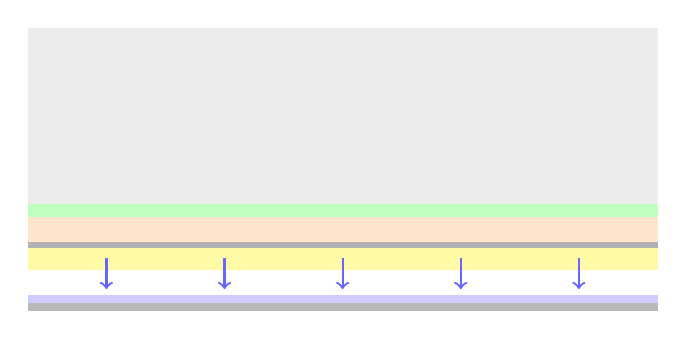
\begin{tikzpicture}[x=1mm,y=2mm]
  \fill[gray!15] (0,0) rectangle (80,-18);
  \fill[gray!55] (0,-18) rectangle (80,-17.5);
  \fill[blue!20] (0,-17.5) rectangle (80,-17.0);
  \fill[white] (0,-17.0) rectangle (80,-15.4);
  \fill[yellow!35] (0,-15.4) rectangle (80,-14.0);
  \fill[gray!60] (0,-14.0) rectangle (80,-13.6);
  \fill[orange!20] (0,-13.6) rectangle (80,-12.0);
  \fill[green!25] (0,-12.0) rectangle (80,-11.2);
  \foreach \x in {10,25,40,55,70}{
    \draw[->,blue!60,thick] (\x,-14.6)--(\x,-16.6);
  }
\end{tikzpicture}}
\caption{積層断面の概念図。}
\label{fig:stack}
\end{figure}
